\subsection{Đánh giá mô hình khôi phục câu tiếng Việt}

Mô-đun ghép câu tiếng Việt là một bài toán sinh văn bản có cấu trúc. Vì vậy, nếu chỉ dùng
một metric duy nhất sẽ khó phản ánh đầy đủ chất lượng đầu ra. Trong báo cáo này, phần
đánh giá cần kết hợp cả \textit{metric huấn luyện} và \textit{metric tương đồng văn bản}:
\begin{itemize}
    \item \textbf{Loss} và \textbf{Perplexity} phản ánh mô hình học phân phối token tốt đến
    mức nào;
    \item \textbf{Exact Match} đo tỉ lệ câu dự đoán trùng hoàn toàn với câu tham chiếu;
    \item \textbf{BLEU} đo mức trùng khớp n-gram sửa đổi giữa câu sinh ra và câu chuẩn;
    \item \textbf{ROUGE-L} nhấn mạnh chuỗi con chung dài nhất, phù hợp khi muốn nhìn cấu
    trúc câu;
    \item \textbf{chrF} đo mức tương đồng ở cấp ký tự, hữu ích với tiếng Việt vì còn liên quan
    tới dấu và biến thể chính tả;
    \item \textbf{Token F1} và \textbf{Similarity Ratio} giúp nhìn thêm ở mức từ và mức chuỗi
    tổng quát.
\end{itemize}

Việc dùng đồng thời các metric trên là phù hợp với các nghiên cứu \textit{Gloss-to-Text}
gần đây, nơi người ta thường không chỉ báo cáo BLEU mà còn bổ sung ROUGE và chrF để
đánh giá nhiều khía cạnh của câu sinh ra.

\subsubsection{Ý nghĩa của từng nhóm metric}

\begin{table}[H]
\centering
\caption{Ý nghĩa của các metric dùng cho mô-đun ghép câu tiếng Việt}
\begin{tabularx}{\textwidth}{|p{3cm}|X|X|}
\hline
\textbf{Metric} & \textbf{Ý nghĩa} & \textbf{Cách diễn giải} \\
\hline
Test Loss & Sai số trung bình khi dự đoán token trên tập test. & Càng thấp càng tốt. \\
\hline
Perplexity & Độ khó dự đoán chuỗi đích của mô hình. & Càng gần 1 càng tốt. \\
\hline
Exact Match & Tỉ lệ câu dự đoán trùng hoàn toàn với câu chuẩn. & Phản ánh độ đúng tuyệt đối. \\
\hline
BLEU & Độ trùng n-gram giữa câu sinh ra và câu tham chiếu. & Phản ánh mức gần giống ở cấp cụm từ. \\
\hline
ROUGE-L & Độ dài chuỗi con chung dài nhất giữa hai câu. & Hữu ích khi quan tâm cấu trúc câu. \\
\hline
chrF & Độ giống nhau ở cấp ký tự. & Nhạy với dấu tiếng Việt và lỗi chính tả nhỏ. \\
\hline
Token F1 & Độ trùng token giữa dự đoán và tham chiếu. & Cân bằng precision và recall theo từ. \\
\hline
Similarity Ratio & Độ tương đồng chuỗi ở mức tổng quát. & Hỗ trợ nhìn nhanh mức độ gần giống. \\
\hline
\end{tabularx}
\end{table}

\begin{figure}[H]
\centering
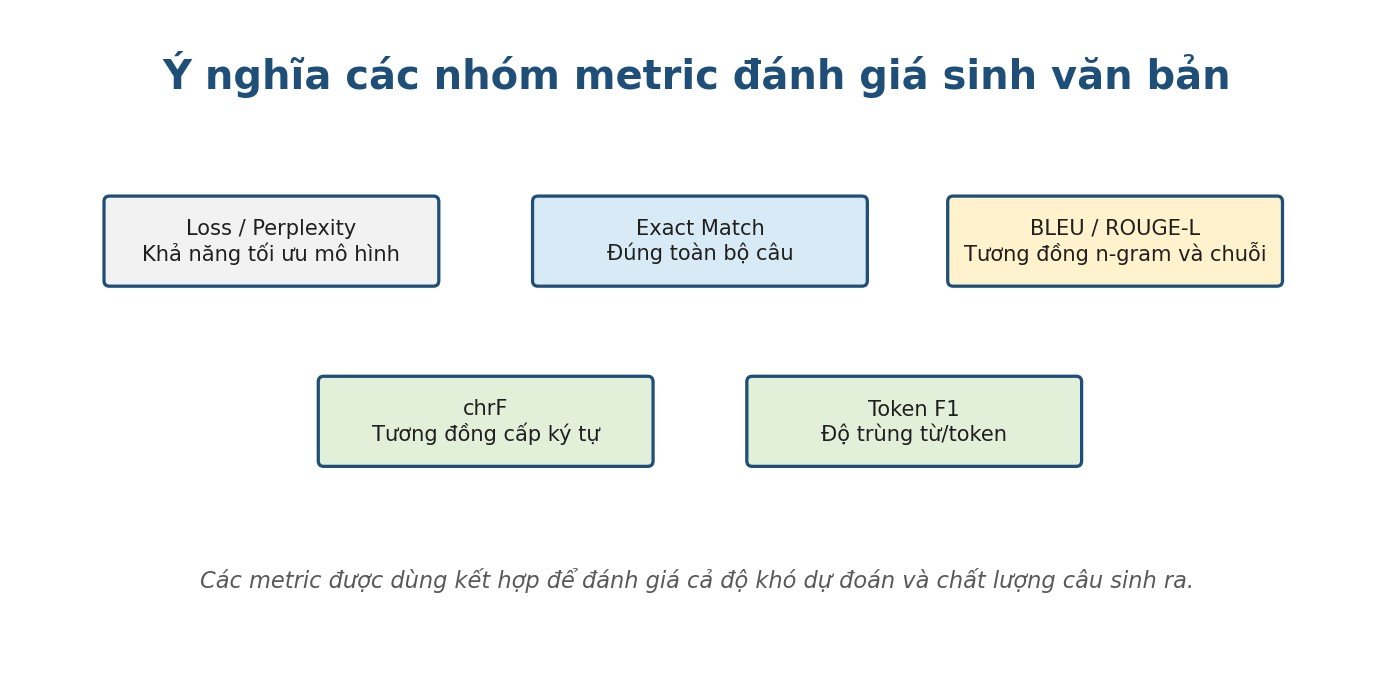
\includegraphics[width=0.82\textwidth]{figures/nlp/vsl_metric_groups.jpg}
\caption{Nhóm ý nghĩa của các metric đánh giá sinh văn bản}
\label{fig:vsl-metric-groups}
\end{figure}

\subsubsection{Kết quả thực nghiệm trên tập test}

Theo báo cáo kỹ thuật của mô-đun \texttt{VSL\_Vietnamese\_NLP}, BARTpho được đánh giá
trên 3.276 mẫu của tập test và cho kết quả như Bảng~\ref{tab:vietnamese-nlp-results}.
Các số liệu này được lấy trực tiếp từ thư mục output của project:
\codepath{VSL_Vietnamese_NLP/outputs/reports/bartpho_sentence_reports/}. Trong đó,
\codepath{bartpho_sentence_metrics_full.json} lưu metric tổng hợp,
\codepath{bartpho_sentence_predictions_full.csv} lưu toàn bộ dự đoán trên tập test và
\codepath{bartpho_sentence_sample_predictions_full.txt} lưu các mẫu dự đoán dễ đọc. Các
giá trị metric này cũng trùng với phần đánh giá trong tài liệu \texttt{vsl.pdf}, mục kết quả
BARTpho trên tập test của module ghép gloss thành câu tiếng Việt.

\begin{table}[H]
\centering
\caption{Kết quả đánh giá mô-đun ghép câu tiếng Việt trên tập test}
\label{tab:vietnamese-nlp-results}
\begin{tabularx}{\textwidth}{|X|c|}
\hline
\textbf{Metric} & \textbf{Giá trị} \\
\hline
Số mẫu test & 3.276 \\
\hline
Test Loss & 0,0040 \\
\hline
Perplexity & 1,0040 \\
\hline
Exact Match & 0,9942 \\
\hline
BLEU & 99,7848 \\
\hline
ROUGE-L & 0,9990 \\
\hline
chrF & 99,8693 \\
\hline
Token F1 & 0,9980 \\
\hline
Similarity Ratio & 0,9991 \\
\hline
\textbf{Exact Match đúng/sai} & \textbf{3.257 / 19} \\
\hline
\end{tabularx}
\end{table}

\begin{figure}[H]
\centering
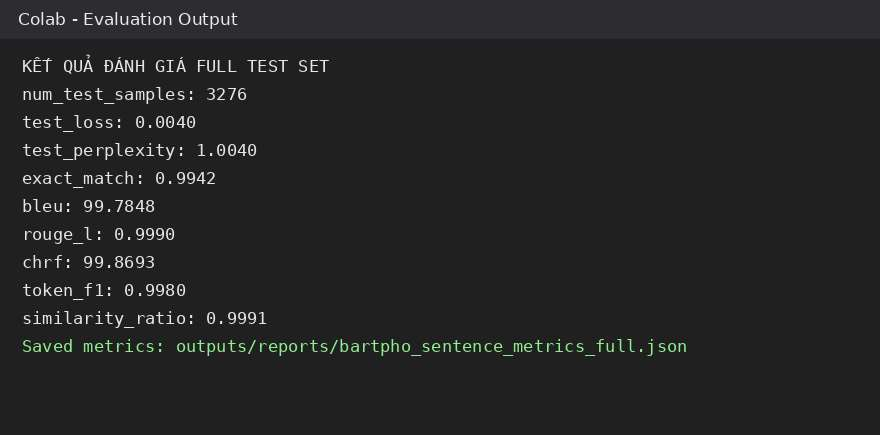
\includegraphics[width=0.78\textwidth]{figures/nlp/vsl_full_test_output.jpg}
\caption{Kết quả đánh giá tự động trên toàn bộ tập test}
\label{fig:vsl-full-test-output}
\end{figure}

\begin{figure}[H]
\centering
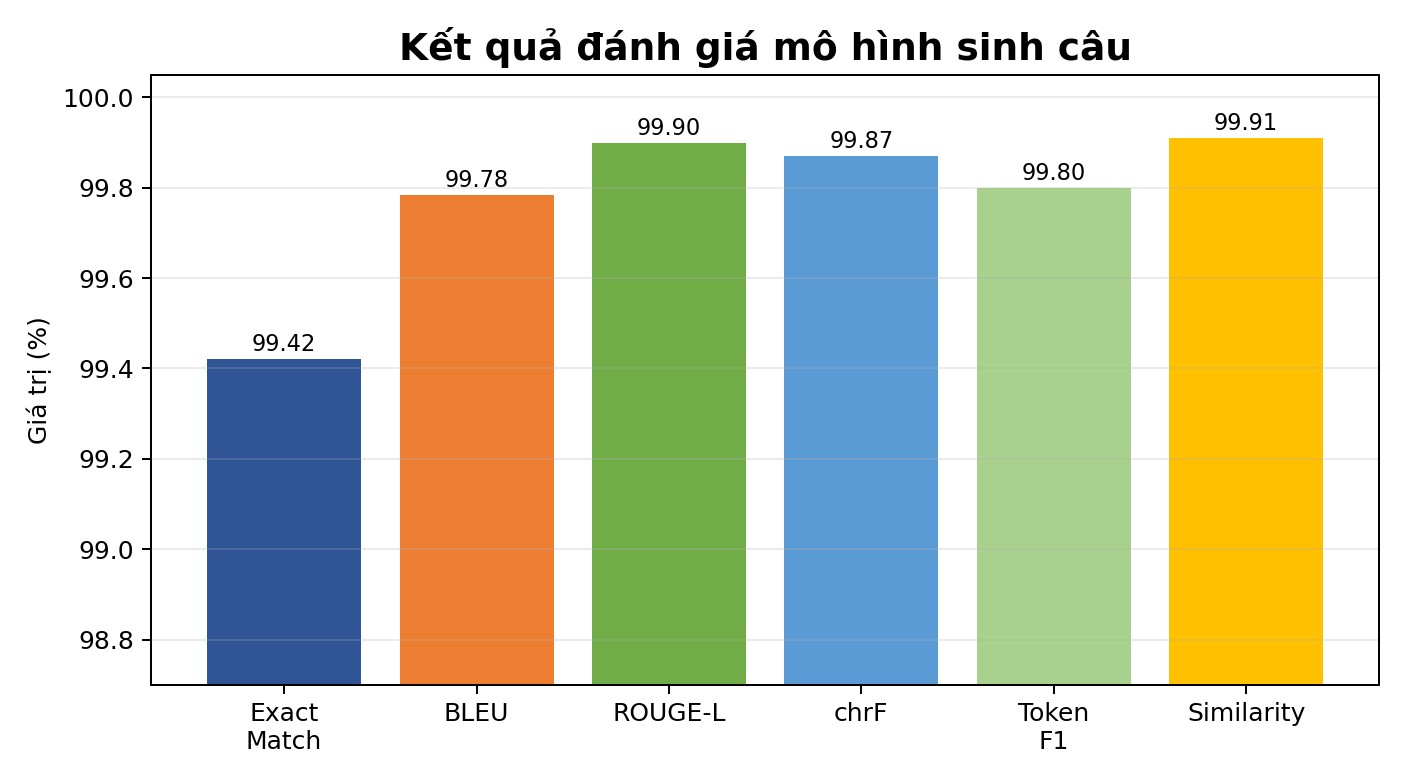
\includegraphics[width=0.9\textwidth]{figures/nlp/vsl_bartpho_metrics_chart.jpg}
\caption{Biểu đồ các metric đánh giá BARTpho trên tập test}
\label{fig:vsl-bartpho-metrics-chart}
\end{figure}

\begin{figure}[H]
\centering
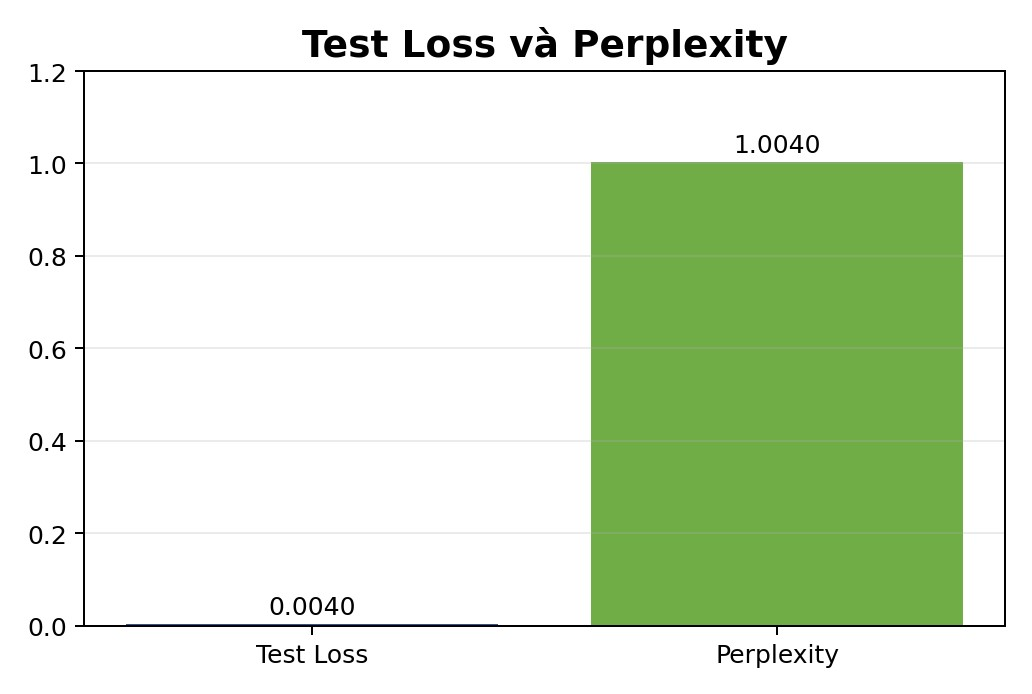
\includegraphics[width=0.72\textwidth]{figures/nlp/vsl_bartpho_loss_perplexity_chart.jpg}
\caption{Biểu đồ Test Loss và Perplexity của BARTpho}
\label{fig:vsl-bartpho-loss-perplexity-chart}
\end{figure}

\subsubsection{Phân tích kết quả}

Các con số trên cho thấy mô hình hoạt động rất tốt trên bộ test hiện tại. Có thể rút ra một
số nhận xét chính:
\begin{itemize}
    \item \textbf{Exact Match = 0,9942} cho thấy gần như toàn bộ câu dự đoán trùng hoàn
    toàn với câu chuẩn. Với một tác vụ có miền dữ liệu giao tiếp tương đối hẹp, đây là tín
    hiệu rất mạnh cho thấy mô hình đã học tốt cấu trúc ánh xạ từ gloss sang câu.
    \item \textbf{BLEU = 99,7848} và \textbf{ROUGE-L = 0,9990} cho thấy câu sinh ra gần
    như trùng khớp hoàn toàn với câu tham chiếu cả ở mức n-gram lẫn cấu trúc chuỗi.
    \item \textbf{chrF = 99,8693} đặc biệt quan trọng với tiếng Việt vì chứng tỏ mô hình giữ
    được dấu và hình thức ký tự rất tốt.
    \item \textbf{Perplexity = 1,0040} cho thấy mô hình gần như không còn nhiều bất định
    trên tập test, phù hợp với việc dữ liệu đầu ra có cấu trúc khá ổn định.
\end{itemize}

Bảng~\ref{tab:vietnamese-nlp-error-samples} trích một số mẫu chưa khớp hoàn toàn từ file dự đoán đầy đủ. Các lỗi này giúp nhìn rõ hơn bản chất sai số
còn lại: đa số là lỗi dấu, nhầm từ gần âm, mất một thành phần ngắn hoặc nhầm mẫu chào hỏi.

\begin{table}[H]
\centering
\caption{Một số mẫu lỗi của mô-đun ghép câu tiếng Việt}
\label{tab:vietnamese-nlp-error-samples}
\begin{tabularx}{\textwidth}{|p{3.4cm}|X|X|}
\hline
\textbf{Gloss} & \textbf{Câu chuẩn} & \textbf{Câu dự đoán} \\
\hline
\texttt{tam\_biet} & Tạm biệt. & Tối nay. \\
\hline
\texttt{xin\_loi} & Tôi xin lỗi. & Xin chào. \\
\hline
\texttt{cam\_on} & Cảm ơn bạn. & Cảm ơn. \\
\hline
\texttt{me di tau\_hoa} & Mẹ đi tàu hỏa. & Mẹ đi tàu. \\
\hline
\texttt{ban can giay} & Bạn cần giấy. & Bạn cần giày. \\
\hline
\texttt{ban dong\_y} & Bạn đồng ý. & Bàn đồng ý. \\
\hline
\end{tabularx}
\end{table}

Nếu chỉ nhìn vào con số, đây là một kết quả gần mức bão hòa. Tuy nhiên, cần đọc đúng bối
cảnh của bộ dữ liệu. Theo mô tả trong báo cáo gốc, \textit{VSL Vietnamese NLP Dataset
v4 Mega} là một \textit{silver dataset} sinh từ rule và template ở nhiều ngữ cảnh khác
nhau. Vì vậy, metric cao phản ánh rất tốt khả năng học lại mẫu câu trong miền dữ liệu đã
thiết kế, nhưng chưa đủ để khẳng định mô hình sẽ đạt chất lượng tương đương trên dữ liệu
giao tiếp tự do ngoài miền.

\subsubsection{Đánh giá định tính và rủi ro diễn giải}

Với một hệ thống ứng dụng, cần bổ sung thêm đánh giá định tính bên cạnh metric tự động.
Ba tiêu chí nên dùng khi xem mẫu dự đoán gồm:
\begin{itemize}
    \item \textbf{Đúng nghĩa}: câu có giữ đúng nhu cầu hoặc trạng thái được biểu diễn bởi
    chuỗi gloss không;
    \item \textbf{Đúng ngữ pháp}: câu có đầy đủ thành phần và đúng trật tự tiếng Việt không;
    \item \textbf{Độ tự nhiên}: câu có giống cách người thật thường nói trong ngữ cảnh tương
    ứng không.
\end{itemize}

Trong trường hợp của project này, metric rất cao là một tín hiệu tốt để chứng minh mô-đun
NLP hoạt động ổn định và có thể tích hợp vào pipeline chung. Tuy nhiên, khi viết kết luận,
nên nhấn mạnh rằng đây là chất lượng đạt được trên bộ dữ liệu có cấu trúc rõ ràng; để
khẳng định năng lực tổng quát hóa mạnh hơn, cần thêm tập kiểm thử người thật hoặc dữ
liệu gloss được sinh từ tầng nhận diện ký hiệu trong điều kiện thực tế.

